\input{{/home/lucas/.config/skel/Latex/configplaindocEN.texconf}}

\usepackage{float}

\author{Lucas Haupt, Dennis Oberst, Lena Wilbert, Alexander Koschenko, David Mertens}
\title{Team Organisation PAM3\\ Mobile Hardware Sampler}
\date{\today}

% Style: Sentence Case (only first word in headings capitalized)
% Author: Lucas Haupt

\begin{document}
\maketitle

\section{Specified rules and techniques}

In order to keep a decent project structure and organisation we decided on the following:

\begin{itemize}
	\item Using a platform to keep an overview over the whole project, individual tasks and time everyone spent working on them
	\item Structuring the project into the following parts and preliminary subtasks
	\begin{table}[!h]
	\centering
	\begin{tabular}{l|c|c}
	\textbf{project part} & \textbf{subtasks} & \textbf{people} \\
	\hline
	MIDI and MIDI circuit & -  & Lena, David \\
	Audio & reading/writing from/to RAM and flash storage, playback & Lucas, Dennis \\
	Display & display controls and user interface & Alex, Dennis \\
	\end{tabular}
	\caption{first project structure}\label{tbl:struct}
	\end{table}
	\item First early draft/ideas on how to put things together (fig. \ref{fig:draft})
	\begin{figure}[H]
	\centering
	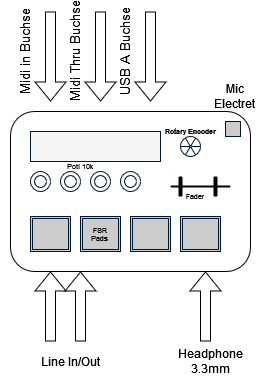
\includegraphics[width=0.5\textwidth]{draft01.png}
	\\
	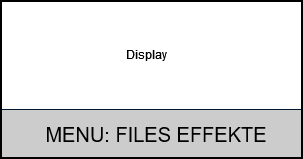
\includegraphics[width=0.5\textwidth]{draft02.png}
	\caption{First draft}\label{fig:draft}
	\end{figure}
\end{itemize}



\section{Things that are still unclear or still to be done}
\begin{itemize}
	\item Reoccuring meetings?
	\item Project goals/milestones (to be included from first presentation)
	\item setting up work management systems with tasks
\end{itemize}

\section{Problems}

\section{Possible approaches to solve them}

\end{document}
